\begin{minipage}[t]{180mm}
\fcolorbox{black}{white}{
\begin{minipage}[b]{30mm}

\includegraphics[width=0.5\linewidth]{unflogo.pdf}
\end{minipage}
\begin{minipage}[b]{100mm}
\Huge \textbf{UNF NEWZ} \\
\Large -- Søvn og retsstavning er overvurderet! 
\end{minipage}
\begin{minipage}[b]{50mm}
\Large Onsdag 17.07.2015 \\
\normalsize Redigeret i \LaTeX\ af \\ SOM, MGS, MMN, SABH
\end{minipage}
}
\end{minipage}



\begin{minipage}[b]{0.95\linewidth}
\begin{minipage}[t]{0.47\textwidth}
\vspace{3mm}
\section*{Produktandmeldelse -- Internettet}


\vspace{1mm}
\section*{Madandmeldelse -- Helstegt spædbarn}
\fcolorbox{black}{white}{$13$ ud af $\aleph_2$ chokoladekiks}
\vspace{2mm}

\section*{Ninjas dagbog}
git status
{\flushright\emph{Ninja, savner sine drab}}

\end{minipage}%
\hfill\begin{minipage}[t]{0.47\textwidth}
\vspace{3mm}
\section*{Vejrudsigt}
\textbf{IMF, AU (fra DMI)}: Skyet med ingen regn og vind fra vest. Op til 20 grader om dagen og ned til 12 grader om natten.

\textbf{JAM}: 3 til 6 grader med svag vind fra nordvest og høj sol. Risiko for isbjørneangreb.

\vspace{-1mm}
\section*{Dagens mediciner}
Hvis du møder en mediciner, så prik hende, og forklar stilfærdig at håndspålægning er den eneste behandling du tror på.

\vspace{-1mm}
\section*{Find en Fynbo}
Under dække af dværgenes angreb, har Fynboen sneget sig ind i dagens avis igen, find ham og smadder hans knæ.

\vspace{-1mm}
\section*{Fakt om Jylland}
Ifølge den jyske metrik er alt under $25$ km gåafstand.

\vspace{-1mm}
\section*{Dagens sandsynlighed}
Sandsynligheden for at en hundværg har skæg er $1$.

\vspace{1mm}
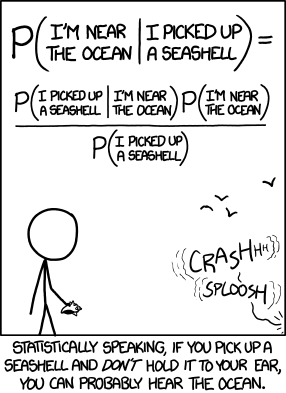
\includegraphics[width=100mm]{seashell.png}
\tiny Randall Munroe, http://xkcd.com/1236/, CC-BY-SA-2.5
\end{minipage}

\begin{center}
\tiny UNF Newz er avisen hvor at ansvarshavende redaktør fralægger sig ethvert ansvar for eventuel plagiering, kaniner, tysk, stavefelj, kaffe, dårlig humor, glemsomhed, katte, store sigmaer, pile, skyer, dårlige oversættelser og alt hvad eventuelle homo sapiens sapiens kunne finde på at holde imod UNF Newz! Dog tager UNF Newz fuld credit og copyright for alle guldkorn, magickort, mus, \TeX, humor, smil, Mortener, kaffe, før-fremtid, ringe og/eller rubik's cube.
\end{center}
\end{minipage}

